\section{Konzeptentwicklungsprozess}
\subsection{Klärung der Aufgabenstellung und Anforderungsanalyse}
\subsubsection{Ziel des Systems}
Ziel des Systems ist es, den Aufbau der Linearführungen für SLC-Positionierer der Baugrößen SLC-17 und SLC-24 so zu gestalten, dass eine spätere voll-Automatisierung möglich ist. Im Vordergrund stehen dabei eine reproduzierbare Vorspannung der Führungen sowie ein kontrollierter Schraubprozess mit definiertem Drehmoment, damit die bisher überwiegend manuelle Montage weniger fehleranfällig, reproduzierbarer und autonom ablaufen kann.

\subsubsection{Randbedingungen}
Die Montage der Linearführungen ist ein qualitätskritischer Arbeitsschritt. Kleine Abweichungen bei der Ausrichtung oder bei der Vorspannung können sich auf die Steifigkeit und das Laufverhalten auswirken. Beim Schraubprozess, wenn das Drehmoment nicht konstant eingehalten wird oder der Schrauber-Bit nicht sauber geführt wird, entstehen Streuungen, die später in der Serienproduktion spürbar werden. Daraus ergibt sich, dass Vorspannung und Verschraubung nicht nur ausgeführt, sondern auch über geeignete Messgrößen überwacht werden müssen.

Eine wichtige technische Randbedingung ist außerdem die Variantenvielfalt. Je nach Ausführung wird die Vorspannung unterschiedlich eingebracht. In den Standardvarianten wird dafür ein bestehendes Vorspannsystem genutzt, das angepasst und in das Gesamtsystem integriert werden muss. Bei den Varianten mit Wand (SLC-W) erfolgt die Vorspannung über Keile, die gezielt eingepresst werden müssen. Zusätzlich muss der Schlitten während des Prozesses zwischenzeitlich bewegt werden, damit der Abstand über die gesamte Länge der Führung gleichmäßig bleibt und keine Verspannungen entstehen.

Organisatorisch muss sich das Konzept in den bestehenden Montageablauf einfügen. Die Arbeit basiert auf Werkstückträgern, und die Schrauben werden vor dem Montageprozess in den vorgesehenen Bohrungen des Führungspakets positioniert. Der Schwerpunkt liegt daher auf einem sauberen, nachvollziehbaren Konzept sowie einer prototypisch umsetzbaren Auslegung, nicht auf einer komplett serienreifen Produktionsanlage. Dennoch soll die Lösung so aufgebaut sein, dass spätere Erweiterungen (z. B. höhere Automatisierung oder bessere Prozessdatenerfassung) möglich bleiben.

\subsubsection{Schnittstellen}
Mechanisch muss das System an den Werkstückträger angebunden sein, auf dem die Bodenplatte bzw. das zu montierende Bauteil positioniert wird. Dazu kommen Schnittstellen zu den Funktionsmodulen, also zur Vorspannmechanik (inklusive Keileinpressen bei SLC-W bzw. Integration des bestehenden Vorspannsystems bei Varianten ohne Wand), zum Schiebesystem für die erforderliche Zwischenbewegung des Schlittens sowie zum Bewegungssystem, das das Schraubwerkzeug präzise an die jeweiligen Schraubpositionen führt. Für die Wiederholbarkeit sind dabei klare Referenzflächen und eine eindeutige Lagefixierung der Bauteile entscheidend.

\begin{figure}[H]
    \centering
    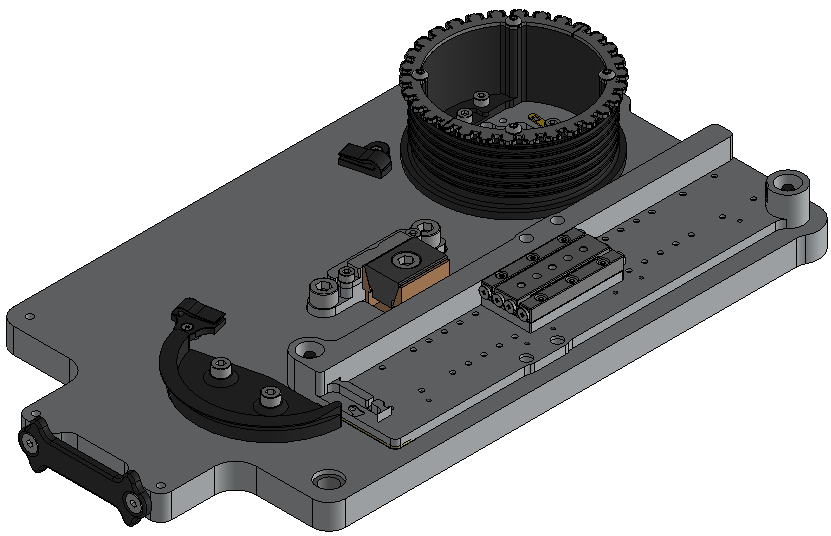
\includegraphics[width=0.5\linewidth]{Bilder/04_Konzeptentwicklung/Schnittstelle.png}
    \caption{Werkstückträger mit SLC2445}
    \label{fig:wst_slc2445}
\end{figure}

Elektrisch und informationstechnisch ergeben sich Schnittstellen zur Ansteuerung der Aktoren, zum Beispiel Achsen für die Schrauberpositionierung, die Schlittenbewegung und den Einpressvorgang. Zusätzlich müssen Sensoren eingebunden werden, um prozessrelevante Größen zu erfassen, insbesondere Drehmoment beim Schraubvorgang und – je nach Konzept – Kraft und Position beim Vorspannen. Die Steuerung muss diese Abläufe koordinieren und Messdaten so bereitstellen, dass die Funktionsweise des Systems im Rahmen von Tests nachvollziehbar überprüft werden kann.

Auf der Mensch-Maschine-Ebene bleibt das Be- und Entladen in der betrachteten Ausbaustufe manuell. Daraus ergibt sich die Anforderung an eine einfache Bedienung mit klaren Funktionen (Start, Stopp, Referenzieren, Quittieren) und einer verständlichen Status- und Fehlerrückmeldung.

\subsubsection{Anforderungsliste}
Die Anforderungen wurden aus der Aufgabenstellung, der Analyse des aktuellen Montageprozesses und den Randbedingungen der Fertigung abgeleitet. Zur besseren Übersicht sind sie in funktionale, mechanische, steuerungstechnische sowie sicherheits- und umgebungsbezogene Anforderungen gegliedert. Zusätzlich wurden sie nach Priorität in MUSS-, SOLL- und KANN-Kriterien eingeteilt. MUSS-Anforderungen dürfen vom späteren Konzept nicht verletzt werden, während SOLL-Anforderungen als Zielwerte dienen und KANN-Anforderungen optionale Verbesserungen darstellen.

Tabelle~\ref{tab:anforderungen_kurz} enthält die für die Konzeptentwicklung relevanten Anforderungen in kompakter Form. Die vollständige Anforderungsliste mit zusätzlichen Angaben (z. B. Nachweis, Kategorie und Kommentare) ist im Anhang~\ref{tab:anforderungsliste} dargestellt. Die Anforderungsliste wird in den folgenden Kapiteln als Grundlage für die Funktionsstruktur, die Bildung der Konzeptvarianten sowie die Bewertung in der Nutzwertanalyse verwendet.

Zur späteren Validierung wurden Anforderungen so formuliert, dass sie überprüfbar sind, z. B. über Maß- und Positionsmessungen, Drehmomentprotokolle oder Zykluszeitmessungen. Wo zum aktuellen Zeitpunkt noch keine konkreten Grenzwerte verfügbar sind, werden diese im Rahmen der konstruktiven Auslegung und der Versuche konkretisiert.\\

{
\small
\renewcommand{\arraystretch}{1.4}
\setlength{\tabcolsep}{12pt}

\begin{longtable}{|p{0.4cm}|p{8.0cm}|p{1.5cm}|p{2.0cm}|}
    \hline
        \textbf{ID} & \textbf{Anforderung (Kurzfassung)} & \textbf{Priorität} & \textbf{Zielwert} \\
    \hline
        \endfirsthead
        \endhead
    \hline
        \endfoot
        \endlastfoot
    
        A01 & Das System muss mit den vorhandenen Werkstückträgern (WST) kompatibel sein. & MUSS & -- \\
    \hline
        A02 & Das System muss die Baugrößen SLC-17 und SLC-24 verarbeiten können. & MUSS & -- \\
    \hline
        A03 & SLC-Positionierer mit Wand (SLC-W) müssen mittels Keile vorgespannt werden können. & MUSS & -- \\
    \hline
        A04 & SLC-Positionierer ohne Wand müssen mit dem bestehenden Vorspannsystem vorgespannt werden. & MUSS & -- \\
    \hline
        A05 & Das Vorspannsystem muss das Führungspaket parallel zur Referenzfläche ausrichten. & MUSS & $\le 20\,\mu\mathrm{m}$ \\
    \hline
        A06 & Die Schrauben sind mit einem vordefinierten Drehmoment anzuziehen. & MUSS & \qty{25}{Ncm} - \qty{60}{Ncm} \\
    \hline
        A26 & Die Positionierabweichung des Schraubwerkzeugs darf in jede Richtung nicht größer als $15\,\mu\mathrm{m}$ sein. & MUSS & $\le 15\,\mu\mathrm{m}$ \\
    \hline
        A11 & Die maximale Systemgröße darf $1200 \times 760\,\mathrm{mm}$ nicht überschreiten. & MUSS & $1200 \times 760\,\mathrm{mm}$ \\
    \hline
        A10 & Die Bearbeitungsdauer pro Positionierer soll unter 5 Minuten liegen. & SOLL & $< 5\,\mathrm{min}$ \\
    \hline
        A22 & Umrüstung zwischen SLC-17 / SLC-24 (mit/ohne Wand) soll schnell und werkzeuglos möglich sein. & SOLL & -- \\
    \hline
    
    \caption{Kernanforderungen für die Konzeptentwicklung}
    \label{tab:anforderungen_kurz}
\end{longtable}
}

\subsubsection{Anforderungserklärung}
Ein Teil der definierten Anforderungen ist nicht lediglich als optionale Verbesserung zu verstehen, sondern entscheidet maßgeblich darüber, ob das System im praktischen Einsatz zuverlässig funktioniert und reproduzierbare Ergebnisse liefert. Die nachfolgend erläuterten Anforderungen sind daher für die spätere Umsetzbarkeit und Bewertung des Konzepts von besonderer Bedeutung.

\begin{itemize}
    \item \textbf{WST-Kompatibilität (A01)} \\
    Die Kompatibilität mit den bestehenden Werkstückträgern stellt eine grundlegende Voraussetzung dar. Abweichungen würden unmittelbare Folgewirkungen nach sich ziehen, etwa Anpassungen an der Zuführung, zusätzliche Aufnahmen oder Umrüstungen in vorgelagerten Systemen. Solche Änderungen wären in der Fertigung nur schwer vermittelbar und würden den wirtschaftlichen Nutzen des Systems deutlich reduzieren. Aus diesem Grund ist diese Anforderung zwingend einzuhalten.

    \item \textbf{Variantenfähigkeit (A02–A04)} \\
    Die Baugrößen SLC-17 und SLC-24 sind als Produktvarianten fest vorgegeben. Zusätzlich stellt die Unterscheidung zwischen Ausführungen mit und ohne Wand unterschiedliche Anforderungen an den Vorspannprozess. Während bei SLC-W-Varianten Keile eingebracht werden müssen, ist bei den übrigen Varianten das bestehende Vorspannsystem zu berücksichtigen. Ein Konzept, das nur eine dieser Varianten abbilden kann, würde im Fertigungsalltag schnell zu einer Insellösung werden. Ziel ist daher eine möglichst flexible Lösung, die alle relevanten Varianten abdeckt.

    \item \textbf{Gleichmäßige Vorspannung (A05)} \\
    Die Einstellung der Vorspannung zählt zu den sensibelsten Schritten im aktuellen Montageprozess. Eine ungleichmäßige Vorspannung über die Führungslänge kann zu einer nicht parallelen Ausrichtung des Führungspakets führen, was lokal erhöhte Reibung oder Überlastungen verursacht und sich negativ auf das Laufverhalten sowie die Lebensdauer des Positionierers auswirkt.  
    Die Vorgabe einer maximalen Parallelitätsabweichung von \enquote{$\leq 20\,\mu\mathrm{m}$} über die gesamte Führungslänge stellt dabei ein eindeutiges und überprüfbares Qualitätskriterium dar.

    \item \textbf{Drehmoment beim Schrauben (A06)} \\
    Das beim Verschrauben eingebrachte Drehmoment steht in direktem Zusammenhang mit der resultierenden Klemmkraft. Schwankungen wirken sich somit unmittelbar auf die Gesamtqualität des Aufbaus aus. Gerade hier bietet eine teilautomatisierte Lösung klare Vorteile, da eine Überwachung und Dokumentation des Drehmoments möglich wird.

    \item \textbf{Positioniertoleranz des Schraubwerkzeugs (A26)} \\
    Die präzise Positionierung des Schraubwerkzeugs ist entscheidend für einen qualitativ hochwertigen Schraubprozess. Ungenaue Werkzeugführung kann zu Schrägansätzen, zusätzlichen Querkräften oder im ungünstigsten Fall zu beschädigten Schraubenköpfen oder Gewinden führen. Die Anforderung einer Positioniertoleranz von \enquote{$\leq 15\,\mu\mathrm{m}$ in alle Richtungen} verdeutlicht, dass es sich hierbei um einen Präzisionsschritt handelt, der dem Qualitätsniveau des Gesamtprodukts entsprechen muss.

    \item \textbf{Bauraum und Budget (A11, A13)} \\
    Die Begrenzung von Bauraum und Kosten definiert den zulässigen Lösungsraum für die Konzeptentwicklung. Der verfügbare Bauraum ist dabei durch die Abmessungen des vorgesehenen ITEM-Arbeitstisches festgelegt, auf dem das System montiert werden soll. Die nutzbare Tischfläche beträgt 1200\,mm $\times$ 760\,mm und stellt eine feste geometrische Randbedingung für den mechanischen Aufbau dar. Alle Baugruppen müssen innerhalb dieser Fläche angeordnet werden, sodass eine sichere Montage, Bedienbarkeit und Integration in die bestehende Fertigungsumgebung gewährleistet sind.\\Zusätzlich begrenzt das zur Verfügung stehende Budget die Auswahl von Komponenten und Lösungsprinzipien. Beide Randbedingungen müssen bereits in einer frühen Phase der Konzeptentwicklung berücksichtigt werden, um technisch realisierbare, wirtschaftlich sinnvolle und in die Fertigung integrierbare Lösungen zu gewährleisten.

    \item \textbf{Prozessdaten und Testskripte (A09, A12)} \\
    Für die Validierung des Systems sowie für eine objektive Bewertung der Prozessstabilität sind geeignete Prozessdaten erforderlich. Ergänzend ermöglichen automatisierte Testskripte eine strukturierte Überprüfung der Steuerungsabläufe und erhöhen die Nachvollziehbarkeit der Ergebnisse. Diese Anforderungen tragen dazu bei, das System nicht nur mechanisch, sondern ganzheitlich zu betrachten.

    \item \textbf{Zykluszeit (A10)} \\
    Die geforderte Zykluszeit von unter fünf Minuten stellt ein sinnvolles Ziel dar, ist jedoch stark vom Automatisierungsgrad und dem verbleibenden manuellen Handling abhängig. Als Soll-Kriterium ist sie realistisch angesetzt und erlaubt es, Qualitäts- und Prozesssicherheitsanforderungen höher zu gewichten, ohne das Gesamtkonzept grundsätzlich infrage zu stellen.
\end{itemize}

\subsection{Funktionsstruktur des Systems}
Ziel der Funktionsstruktur ist es, die Gesamtaufgabe des Systems unabhängig von einer konkreten konstruktiven Lösung zu beschreiben. Durch die Zerlegung in Teilfunktionen wird transparent, welche Funktionen das System erfüllen muss und wie diese logisch miteinander verknüpft sind. Die Funktionsstruktur bildet damit die Grundlage für die nachfolgende Konzeptentwicklung und -bewertung.

\subsubsection{Gesamtfunktion}
Die Gesamtfunktion des Systems besteht darin, Linearführungen der SLC-Positionierer reproduzierbar und qualitätsgesichert zu montieren. Dies umfasst das kontrollierte Vorspannen des Führungspakets, das präzise Verschrauben sowie die Handhabung unterschiedlicher Produktvarianten. Der Prozess soll dabei kompatibel zu bestehenden Werkstückträgern sein, prozessrelevante Daten erfassen und unter definierten Sicherheits- und Randbedingungen ablaufen.\\
Zusammenfassend lässt sich die Gesamtfunktion wie folgt formulieren:
\begin{quote}
\textit{Vorspannen und Verschrauben von SLC-Linearführungen unter kontrollierten Kraft-, Positions- und Drehmomentbedingungen bei gleichzeitiger Variantenfähigkeit und Prozessüberwachung.}
\end{quote}

\subsubsection{Funktionszerlegung}
Zur funktionalen Beschreibung des Systems wird die Gesamtfunktion in übergeordnete Teilfunktionen zerlegt. Ziel dieser Zerlegung ist es, die wesentlichen Aufgaben des Systems strukturiert darzustellen, ohne bereits auf konkrete technische Lösungen einzugehen.

Die Funktionszerlegung orientiert sich am grundsätzlichen Montageablauf der Linearführungen sowie an den identifizierten, qualitätsrelevanten Prozessschritten. Dabei wird zwischen vorbereitenden Funktionen, montagebezogenen Kernfunktionen und abschließenden Funktionen unterschieden.

Der Prozess beginnt mit dem Einlegen und Erkennen des Werkstückträgers. Anschließend erfolgt eine variantenabhängige Vorspannung des Führungspakets, gefolgt vom positionsgenauen Schraubprozess. Nach Abschluss der Montage wird der Werkstückträger entnommen.

Entscheidungen, insbesondere die Unterscheidung zwischen SLC- und SLC-W-Varianten, sind als funktionale Verzweigungen berücksichtigt. Wiederkehrende Abläufe, wie das schrittweise Verschrauben entlang der Führung, werden funktional als Schleifen abgebildet.

Die detaillierte Betrachtung und Bewertung der einzelnen Teilfunktionen erfolgt im Abschnitt~\ref{sec:teilfunktionen}.

\subsubsection{System- und Funktionsstrukturdiagramm}
Der Montageprozess der Linearführung lässt sich als eine klar strukturierte Abfolge einzelner Arbeitsschritte beschreiben. Um diesen Ablauf nachvollziehbar darzustellen, wird ein Funktionsstrukturdiagramm in Form eines Ablaufdiagramms verwendet. Es zeigt den Prozess vom Einlegen des Werkstückträgers bis zur Entnahme des montierten Bauteils.

Der Ablauf folgt der tatsächlichen Reihenfolge der Montage. Entscheidungen, wie die Unterscheidung zwischen SLC- und SLC-W-Varianten, sind als Verzweigungen im Diagramm integriert. Dadurch kann der gleiche grundlegende Ablauf für beide Produktvarianten verwendet werden, ohne separate Prozesse darstellen zu müssen.

Arbeitsschritte, die mehrfach durchlaufen werden, sind als Schleifen ausgeführt. Dies betrifft insbesondere das Einschrauben der Befestigungsschrauben und das anschließende Verschieben des Schlittens, bis alle Schrauben vollständig eingeschraubt sind. Auf diese Weise wird der sequentielle Charakter des Montageprozesses klar erkennbar.

Das Funktionsstrukturdiagramm dient damit als Übersicht über den zeitlichen und logischen Ablauf des Montageprozesses und bildet die Grundlage für die weitere funktionale Betrachtung des Systems.

\begin{figure}[htbp]
    \centering
    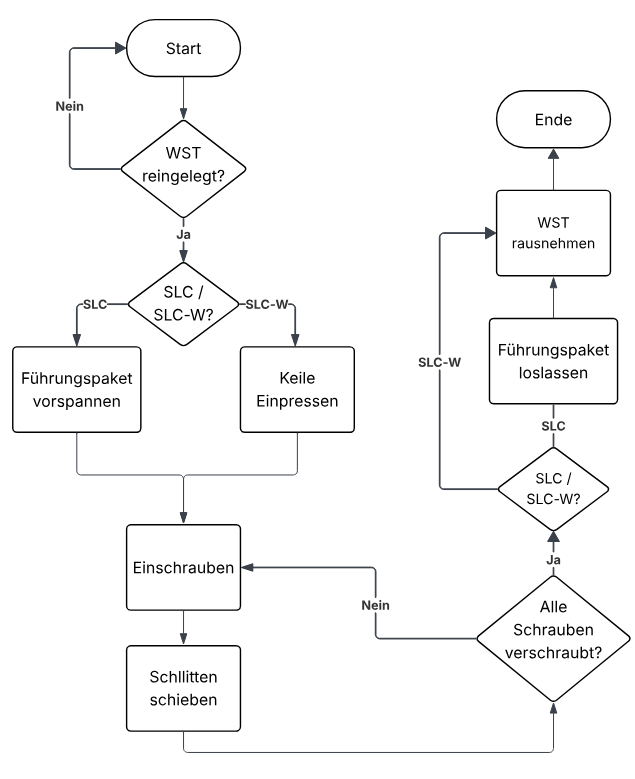
\includegraphics[width=0.48\linewidth]{Bilder/04_Konzeptentwicklung/Flowchart.png}
    \caption{Ablaufsdiagramm des Montageprozesses}
    \label{fig:Flowchart}
\end{figure}

\subsubsection{Strukturelle Funktionsstruktur der Montagesystems}

Neben dem zeitlichen Ablauf ist es für das Verständnis des Systems notwendig, die Montagestation als funktionale Einheit zu betrachten. Zu diesem Zweck wird eine strukturelle Funktionsstruktur verwendet, die das System unabhängig vom zeitlichen Ablauf beschreibt.

In dieser Darstellung ist die Montagestation als abgegrenztes System dargestellt, das mit seiner Umgebung über definierte Ein- und Ausgänge verbunden ist. Innerhalb der Systemgrenze sind die wesentlichen Funktionen zusammengefasst, die zur Umsetzung des Montageprozesses erforderlich sind. Dazu zählen unter anderem das Positionieren und Fixieren des Werkstückträgers, das Vorspannen beziehungsweise Einpressen des Führungspakets, der Schraubprozess sowie die Überwachung und Freigabe einzelner Prozessschritte.

Die strukturelle Funktionsstruktur macht deutlich, welche Funktionen im System realisiert werden und wie diese gemeinsam zur Erfüllung der Gesamtfunktion beitragen. Im Gegensatz zum Ablaufdiagramm wird hier bewusst keine zeitliche Reihenfolge dargestellt. Stattdessen liegt der Fokus auf der funktionalen Gliederung des Systems und der Abgrenzung zur Umgebung.

Die strukturelle Funktionsstruktur stellt damit die Verbindung zwischen dem Ablaufdiagramm und der anschließenden Betrachtung der Informations- und Energieflüsse dar.

\begin{figure}[htbp]
    \centering
    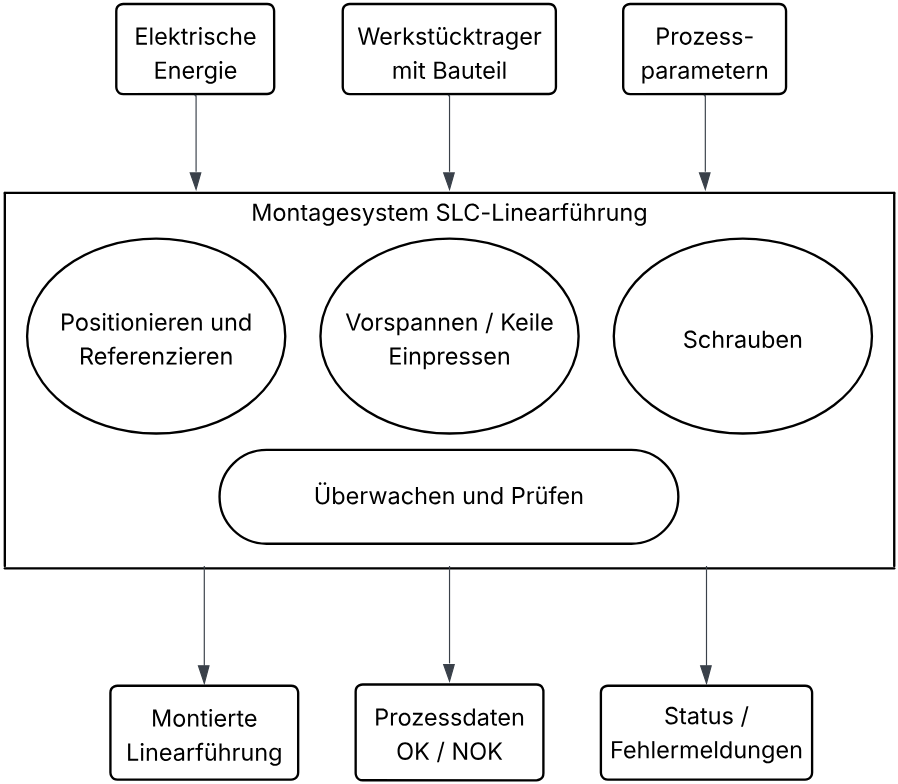
\includegraphics[width=0.45\linewidth]{Bilder/04_Konzeptentwicklung/Strukturelle Funktionsdiagramm.png}
    \caption{Strukturelle Funktionsstruktur des Montagesystems}
    \label{fig:Strukturelle_Funktionsstruktur}
\end{figure}

Die Funktionsstruktur bildet damit die Grundlage für die nachfolgende Konzeptentwicklung und -bewertung.\cite{VDI2221, MKon_VL, PahlBeitz}

\subsection{Lösungsprinzipien und Konzeptvarianten}
\subsubsection{Teilfunktionen}
\label{sec:teilfunktionen}
Aufbauend auf der im vorherigen Abschnitt dargestellten Funktionsstruktur werden im Folgenden die für die Konzeptentwicklung relevanten Teilfunktionen betrachtet. Ziel dieses Abschnitts ist es, diese Teilfunktionen eindeutig zu benennen und voneinander abzugrenzen, sodass sie im weiteren Verlauf gezielt als Grundlage für die Entwicklung technischer Lösungsprinzipien genutzt werden können.

Während die Funktionsstruktur die Aufgaben des Systems bewusst lösungsneutral beschreibt, stellen die Teilfunktionen die Verbindung zwischen der funktionalen Analyse und der späteren technischen Umsetzung dar. Sie konkretisieren die funktionalen Anforderungen soweit, dass darauf aufbauend unterschiedliche Lösungsansätze systematisch entwickelt, verglichen und kombiniert werden können.\cite{VDI2221, MKon_VL}

Die Identifikation der Teilfunktionen erfolgte auf Basis des realen Montageablaufs sowie der zuvor abgeleiteten Anforderungen. Der Schwerpunkt liegt dabei auf den qualitätskritischen Prozessschritten beim Aufbau der Linearführungen. Insbesondere die reproduzierbare Vorspannung des Führungspakets, der kontrollierte Schraubprozess sowie die übergeordnete Steuerung und Prozessüberwachung stehen im Fokus der Betrachtung.

Zur besseren Übersicht sind die identifizierten Haupt-, Unter- und Teilfunktionen in Tabelle~\ref{tab:teilfunktionen} strukturiert zusammengefasst. Zusätzlich ist der Bezug zu den jeweiligen Anforderungen angegeben. Die Tabelle dient als funktionale Orientierung für die nachfolgende Konzeptentwicklung und ermöglicht eine klare Zuordnung der späteren Lösungsprinzipien zu den einzelnen Teilfunktionen. Die inhaltliche Erläuterung der wesentlichen Teilfunktionen erfolgt im Anschluss.

{
\small
\setlength{\tabcolsep}{6pt}
\renewcommand{\arraystretch}{1.2}

\begin{longtable}{|p{0.5cm}|p{2.5cm}|p{0.6cm}|p{3.5cm}|p{0.8cm}|p{5.0cm}|}
\hline
\textbf{Nr.} & \textbf{Hauptfunktion} &
\textbf{Nr.} & \textbf{Unterfunktion} &
\textbf{Nr.} & \textbf{Teilfunktion} \\
\hline
\endfirsthead
\endhead
\hline
\endfoot
\endlastfoot

1 & Führungspaket vorspannen (SLC) & 1.1 & Werkstückaufnahme &
1.1.1 & Kompatibilität mit Werkstückträgern sicherstellen (A01) \\
\cline{3-6}
  &  & 1.2 & Baugrößenerkennung &
1.2.1 & SLC-17 / SLC-24 erkennen und umstellen (A02) \\
\cline{3-6}
  &  & 1.3 & Vorspannkraft einbringen &
1.3.1 & Gleichmäßige Vorspannung über die Länge sicherstellen (A05) \\
\cline{3-6}
  &  & 1.4 & Maßhaltigkeit sichern &
1.4.1 & Toleranzen beim Führungseinbau einhalten (A13) \\
\hline

2 & Einklappfedern einpressen (SLC-W) & 2.1 & Federvorspannung erzeugen &
2.1.1 & Einklappfedern bei SLC mit Wand einpressen (A03) \\
\cline{3-6}
  &  & 2.2 & Positionierung des Feder-Drückteils &
2.2.1 & Feder-Drückteil definiert zur Einklappfeder ausrichten und positionieren (A04) \\
\hline

3 & Schraubprozess & 3.1 & Schrauben eindrehen &
3.1.1 & Schrauben mit definiertem Drehmoment anziehen (A06) \\
\cline{3-6}
  &  & 3.2 & Werkzeugführung &
3.2.1 & Schraubwerkzeug präzise positionieren (A07) \\
\hline

4 & Steuerung und Prozessüberwachung & 4.1 & Montageablauf steuern &
4.1.1 & Steuerung aus Hardware und Software auswählen und implementieren (A08) \\
\cline{3-6}
  &  & 4.2 & Steuerungsvalidierung &
4.2.1 & Testskripte entwickeln und Abläufe prüfen (A09) \\
\cline{3-6}
  &  & 4.3 & Prozessüberwachung &
4.3.1 & Positions-, Drehmoment- und Prozessdaten erfassen (A11, A15) \\
\cline{3-6}
  &  & 4.4 & Bedien- und Umrüstschnittstelle &
4.4.1 & Umrüstung zwischen SLC-17 und SLC-24 ermöglichen (A21) \\
\cline{3-6}
  &  & 4.5 & Sollzeitgerechte Auslegung &
4.5.1 & Einhaltung der Soll-Bearbeitungszeit (A25) \\
\hline

5 & Wartung und Erweiterbarkeit & 5.1 & Wartungsfreundlichkeit &
5.1.1 & Wartungsarm gestalten (A19) \\
\cline{3-6}
  &  & 5.2 & Erweiterbarkeit &
5.2.1 & System für neue Baugrößen vorbereiten (A20) \\
\hline

6 & Optionale Systemmerkmale & 6.1 & Energieeffizienz &
6.1.1 & Energieverbrauch optimieren (A23) \\
\cline{3-6}
  &  & 6.2 & Transportfähigkeit &
6.2.1 & System auf Rollen oder modular zerlegbar gestalten (A24) \\
\hline

\caption{Übersicht der Haupt-, Unter- und Teilfunktionen des Montagesystems}
\label{tab:teilfunktionen}
\end{longtable}
}

\begin{enumerate}
    \item \textbf{Führungspaket vorspannen}\\
    Ziel dieser Hauptfunktion ist es, eine definierte und reproduzierbare Vorspannung über die gesamte Länge der Linearführung sicherzustellen.

    Hierfür sind insbesondere folgende Teilfunktionen erforderlich:
    \begin{itemize}
        \item \textbf{Gleichmäßige Vorspannkraft erzeugen}\\
        Sicherstellung einer gleichmäßigen Kraftverteilung entlang der Führung, um eine parallele Ausrichtung des Führungspakets zur Referenzfläche zu gewährleisten.

        \item \textbf{Vorspannelement in Richtung SLC bewegen}\\
        Gezielte, geführte Bewegung eines Vorspannelements zur kontrollierten Einbringung der erforderlichen Vorspannkraft.

        \item \textbf{Einklappfedern einpressen (SLC-W)}\\
        Variantenabhängige Erzeugung der Vorspannung durch das kontrollierte Einpressen der Einklappfedern bei SLC-Positionierern mit Wand.
        \begin{itemize}
            \item \textbf{Position der Feder erfassen}\\
            Überwachung der Lage der Einklappfeder während des Einpressvorgangs.
            \item \textbf{Einpresskraft einstellen}\\
            Anpassung der Einpresskraft zur Vermeidung von Beschädigungen und zur Sicherstellung reproduzierbarer Ergebnisse.
        \end{itemize}
    \end{itemize}
    
    \item \textbf{Schraubprozess}\\
    Der Schraubprozess dient der form- und kraftschlüssigen Fixierung der Linearführung in der vorgespannten Position. Die Prozessqualität hängt dabei wesentlich von der präzisen Positionierung des Schraubwerkzeugs sowie von der kontrollierten Einbringung des Drehmoments ab.

    Die hierfür relevanten Teilfunktionen sind:
    \begin{itemize}
        \item \textbf{Position der Schrauben erfassen}\\
        Bestimmung der jeweiligen Schraubpositionen als Grundlage für eine präzise Werkzeugführung.

        \item \textbf{Schraubwerkzeug positionieren}\\
        Exaktes Anfahren der Schraubpositionen innerhalb der vorgegebenen Toleranzen.

        \item \textbf{Drehmoment einstellen und überwachen}\\
        Sicherstellung eines definierten Drehmoments während des Einschraubvorgangs.

        \item \textbf{Schraubtiefe erfassen}\\
        Kontrolle der Einschraubtiefe als zusätzliches Qualitätsmerkmal.

        \item \textbf{Schlitten schieben}\\
        Inkrementelle Bewegung des Schlittens entlang der Führung, um den Schraubprozess schrittweise über die gesamte Führungslänge durchführen zu können.
    \end{itemize}

    \item \textbf{Steuerung und Prozessüberwachung}\\
    Die Steuerung koordiniert alle Teilfunktionen und stellt sicher, dass der Montageprozess in der vorgesehenen Reihenfolge und unter Einhaltung der definierten Randbedingungen abläuft. Zusätzlich übernimmt sie Aufgaben der Prozessüberwachung sowie der Datenerfassung.

    Zentrale Teilfunktionen in diesem Bereich sind:
    \begin{itemize}
        \item \textbf{Subsysteme kalibrieren}\\
        Kalibrierung von Sensoren und Referenzierung von Aktoren zur Sicherstellung reproduzierbarer Prozessbedingungen.

        \item \textbf{Montageprozess steuern}\\
        Ablaufsteuerung der einzelnen Prozessschritte einschließlich Variantenentscheidung und Fehlerbehandlung.
    \end{itemize}
\end{enumerate}

\textbf{Zusammenfassung und Überleitung}\\
Die beschriebenen Teilfunktionen bilden die funktionale Grundlage für die nachfolgende Entwicklung technischer Lösungsprinzipien. In den folgenden Abschnitten werden für ausgewählte Teilfunktionen unterschiedliche Lösungsansätze untersucht und zu konsistenten Konzeptvarianten zusammengeführt.

\subsubsection{Lösungsprinzipien für Teilfunktionen}
\label{sec:teilfuktionenlösungen}
Für die in Abschnitt~\ref{sec:teilfunktionen} definierten Teilfunktionen wurden jeweils mehrere technische Lösungsprinzipien identifiziert. Ziel dieses Abschnitts ist es, die möglichen Umsetzungsansätze pro Teilfunktion übersichtlich darzustellen, ohne diese bereits zu einem Gesamtkonzept zu kombinieren oder zu bewerten.\cite{MKon_VL, PahlBeitz, ZwickyMorphology}

Die Lösungsprinzipien wurden auf der Basis des bestehenden Montageprozesses, der technischen Machbarkeit sowie der definierten Anforderungen erarbeitet. Dabei wurden sowohl einfach ausgestaltete, robuste Lösungen als auch stärker automatisierte Ansätze berücksichtigt, um ein breites Lösungsspektrum abzudecken.

Für die Werkstückaufnahme wurden sowohl manuelle Einlegekonzepte als auch automatisierte Varianten, beispielsweise mittels eines 6-achsen-Roboters, betrachtet. Die Sicherung des Werkstücks kann mechanisch über Spannvorrichtungen mit Passstiften oder alternativ über Vakuumbasierte Systeme erfolgen.

Im Bereich der Baugrößenumschaltung reichen die Lösungsansätze von einer manuellen Eingabe über das automatische Einlesen eines Codes bis hin zu sensor- oder kamerabasierten Erkennungsverfahren. Das Vorspannsystem kann entweder auf einem bereits bestehenden mechanischen System aufbauen oder durch zusätzliche Aktorik ergänzt werden.

Zur Erfassung der Schlittenposition wurden verschiedene sensorische Prinzipien untersucht, darunter geführte Bewegungen bis zum Werkstückanschlag, Laser-Triangulations\-sensoren, kamerabasierte Systeme sowie ToF-Sensorik. Für die Bewegung des Schraubwerkzeugs wurden kartesische Systeme wie XYZ- oder Gantry-Achsen ebenso betrachtet wie robotische Lösungen mit höherer Bewegungsfreiheit.

Beim Einschraubsystem wurden sowohl einfache manuelle Schraubwerkzeuge als auch drehmomentgeregelte industrielle Schrauber untersucht. Ergänzend wurden unterschiedliche Konzepte für den Endeffektor, die Positionsüberwachung, das Steuerungssystem sowie Sicherheits-, Transport- und Energieeffizienzaspekte betrachtet.\\\\

{
\small
\setlength{\tabcolsep}{4pt}
\renewcommand{\arraystretch}{1.2}

\begin{tabularx}{\textwidth}{|p{3.5cm}|X|X|X|X|}
\hline
\textbf{Teilfunktion} & \multicolumn{4}{c|}{\textbf{Lösungsprinzipien}} \\
\hline
\endfirsthead
\endhead
\hline
\endfoot
\endlastfoot

WST-Aufnahme & Manuelle Einsetzung & Einsetzung durch Cobot & -- & -- \\
\hline
WST-Sicherung & Spannvorrichtung mit Stiften & Vakuum\-aufnahme & -- & -- \\
\hline
Baugrößen\-identifikation & Automatisches Code-Scannen & Manuelle Eingabe & Sensor- oder bildbasierte Erkennung & -- \\
\hline
Vorspannsystem & Bestehendes mechanisches Vorspannsystem & -- & -- & -- \\
\hline
Schlittenposition erfassen & Geführte Bewegung bis Werkstückanschlag & Laser-Triangulations- / IR-Sensor & Kamera & ToF-Sensor \\
\hline
Schrauber\-bewegungssystem & XYZ-Achsensystem & Gantry-System & 6-Achs-Roboter & SCARA / Pick-and-Place \\
\hline
Einklappfedern einpressen & Hydraulische Presse & Ventilgesteuerte Presse & Motor\-angetriebener Stift & -- \\
\hline
Einschraubsystem & Konventioneller Schraubendreher mit drehbarem Endeffektor & Drehmoment\-geregelter Schrauber (z.\,B. MITO15CA + EDU 2AE) & -- & -- \\
\hline
Schiebersystem & Aufsteckbares Gummipad mit manueller Presse & Gummiauflage auf Hülse & Gummistift & -- \\
\hline
Endeffektor & Einfacher Greifer & Kombinierter Endeffektor & Mehrfach-Endeffektor & -- \\
\hline
Positions\-überwachung & Encoder & Schrittzähler & Distanzsensoren & Bildverarbeitung \\
\hline
Steuerungssystem & SPS-basierte Steuerung & IPC-basiertes Motion-Control-System & Industrie-Robotercontroller & -- \\
\hline
Transportfähigkeit & Fix montiert & Rollen mit Feststeller & Modular zerlegbar & -- \\
\hline
Energieeffizienz & Intelligente Abschaltung bei Inaktivität & Keine Optimierung & Energiesparende Antriebe & -- \\
\hline

\caption{Übersicht der Lösungsprinzipien für die einzelnen Teilfunktionen}
\label{tab:loesungsprinzipien_teilfunktionen}
\end{tabularx}
}

Die Gesamtheit dieser Lösungsprinzipien ist im morphologischen Kasten strukturiert dargestellt und bildet die Grundlage für die nachfolgende Bildung von Konzeptvarianten.

\subsubsection{Bildung von Konzeptvarianten}
Zur Bildung konsistenter Gesamtkonzepte wurden die in Abschnitt~\ref{sec:teilfuktionenlösungen} dargestellten Lösungsprinzipien mithilfe eines morphologischen Kastens systematisch kombiniert. Der morphologische Kasten stellt für jede Teilfunktion mehrere alternative Lösungsansätze gegenüber und ermöglicht es, diese gezielt zu vollständigen Konzeptvarianten zusammenzuführen.

Eine Konzeptvariante entsteht dabei durch die Auswahl genau eines Lösungsprinzips pro Teilfunktion. Durch das Verbinden dieser ausgewählten Lösungen im morphologischen Kasten ergeben sich zusammenhängende Linien, die jeweils ein in sich geschlossenes Gesamtkonzept repräsentieren.

Bei der Auswahl der Kombinationen wurde darauf geachtet, dass die einzelnen Lösungsprinzipien technisch kompatibel sind und gemeinsam einen vollständigen Montageprozess abbilden. Gleichzeitig wurden bewusst unterschiedliche Automatisierungsgrade realisiert, um im weiteren Verlauf einen vergleichenden Ansatz zu ermöglichen.

Auf diese Weise wurden mehrere Konzeptvarianten definiert, die sich hinsichtlich Systemkomplexität, Automatisierungsgrad und technischer Ausprägung unterscheiden. Diese Varianten bilden die Grundlage für die nachfolgende detaillierte Beschreibung und Bewertung.
\\\\\\\\

\begin{center}
\small
\renewcommand{\arraystretch}{1.4}
\setlength{\tabcolsep}{12pt}
\begin{tabular}{|c|c|}
    \hline
    \textbf{Konzept} & \textbf{Linienmuster} \\
    \hline
    \textbf{A} &
    \textcolor{conceptA}{\rule{2.5cm}{0.8pt}} \\
    \hline
    \textbf{B} &
    \textcolor{conceptB}{
        \rule[0.3ex]{0.5cm}{0.8pt}\hspace{0.2cm}
        \rule[0.3ex]{0.5cm}{0.8pt}\hspace{0.2cm}
        \rule[0.3ex]{0.5cm}{0.8pt}
    } \\
    \hline
    \textbf{C} &
    \textcolor{conceptC}{
        \rule[0.3ex]{0.15cm}{0.8pt}\hspace{0.15cm}
        \rule[0.3ex]{0.15cm}{0.8pt}\hspace{0.15cm}
        \rule[0.3ex]{0.15cm}{0.8pt}\hspace{0.15cm}
        \rule[0.3ex]{0.15cm}{0.8pt}\hspace{0.15cm}
        \rule[0.3ex]{0.15cm}{0.8pt}\hspace{0.15cm}
        \rule[0.3ex]{0.15cm}{0.8pt}
    } \\
    \hline
\end{tabular}
\end{center}
\clearpage

\begin{comment}
{
\small
\setlength{\tabcolsep}{4pt}
\renewcommand{\arraystretch}{1.2}

\begin{tabularx}{\textwidth}{|p{3.5cm}|X|X|X|X|}
\hline
\textbf{Teilfunktion} & \multicolumn{4}{c|}{\textbf{Lösungsprinzipien}} \\
\hline

WST-Aufnahme
& Manuelle Einsetzung \cellnode{wst_man}
& Einsetzung durch Cobot \cellnode{wst_cobot}
& -- & -- \\
\hline

WST-Sicherung
& Spannvorrichtung mit Stiften \cellnode{sich_stift}
& Vakuum\-aufnahme \cellnode{sich_vak}
& -- & -- \\
\hline

Baugrößen\-identifikation
& Automatisches Code-Scannen \cellnode{id_code}
& Manuelle Eingabe \cellnode{id_man}
& Sensor- oder bildbasierte Erkennung \cellnode{id_cam}
& -- \\
\hline

Vorspannsystem
& Bestehendes mechanisches Vorspannsystem \cellnode{vorspann}
& -- & -- & -- \\
\hline

Schlittenposition erfassen
& Geführte Bewegung bis Werkstückanschlag \cellnode{pos_anschlag}
& Laser-Triangulations- / IR-Sensor \cellnode{pos_laser}
& Kamera \cellnode{pos_cam}
& ToF-Sensor \cellnode{pos_tof} \\
\hline

Schrauber\-bewegungssystem
& XYZ-Achsensystem \cellnode{move_xyz}
& Gantry-System \cellnode{move_gantry}
& 6-Achs-Roboter \cellnode{move_6ax}
& SCARA / Pick-and-Place \cellnode{move_scara} \\
\hline

Einklappfedern einpressen
& Hydraulische Presse \cellnode{press_hyd}
& Ventilgesteuerte Presse \cellnode{press_valve}
& Servo\-angetriebener Stift \cellnode{press_servo}
& -- \\
\hline

Einschraubsystem
& Konventioneller Schraubendreher \cellnode{screw_simple}
& Drehmoment\-geregelter Schrauber \cellnode{screw_mito}
& -- & -- \\
\hline

Schiebersystem
& Aufsteckbares Gummipad \cellnode{slide_pad}
& Gummiauflage auf Hülse \cellnode{slide_sleeve}
& Gummistift \cellnode{slide_pin}
& -- \\
\hline

Endeffektor
& Einfacher Greifer \cellnode{ee_simple}
& Kombinierter Endeffektor \cellnode{ee_combo}
& Mehrfach-Endeffektor \cellnode{ee_multi}
& -- \\
\hline

Positions\-überwachung
& Encoder \cellnode{ctrl_enc}
& Schrittzähler \cellnode{ctrl_step}
& Distanzsensoren \cellnode{ctrl_dist}
& Bildverarbeitung \cellnode{ctrl_img} \\
\hline

Steuerungssystem
& SPS-basierte Steuerung \cellnode{ctrl_plc}
& IPC-basiert \cellnode{ctrl_ipc}
& Robotercontroller \cellnode{ctrl_robot}
& -- \\
\hline

Transportfähigkeit
& Fix montiert
& Rollen mit Feststeller
& Modular zerlegbar
& -- \\
\hline

Energieeffizienz
& Intelligente Abschaltung
& Keine Optimierung
& Energiesparende Antriebe
& -- \\
\hline

\caption{Übersicht der Lösungsprinzipien für die einzelnen Teilfunktionen}
\label{tab:morphologischer_kasten}
\end{tabularx}
}

\begin{tikzpicture}[remember picture,overlay]

% Beispiel: gewählte Lösung (rot)
\draw[red, very thick]
  (wst_cobot) -- (sich_stift)
  -- (id_code)
  -- (vorspann)
  -- (pos_laser)
  -- (move_xyz)
  -- (press_servo)
  -- (screw_mito)
  -- (slide_pin)
  -- (ee_combo)
  -- (ctrl_enc)
  -- (ctrl_plc);

% Alternative Variante (grün gestrichelt)
\draw[green!60!black, dashed, very thick]
  (wst_man) -- (sich_vak)
  -- (id_cam)
  -- (pos_cam)
  -- (move_gantry)
  -- (press_valve);

\end{tikzpicture}
\end{comment}

\begin{table}[H]
\centering
\small
\setlength{\tabcolsep}{4pt}
\renewcommand{\arraystretch}{1.2}

\begin{tabularx}{\textwidth}{|p{3.5cm}|X|X|X|X|}
\hline
\textbf{Teilfunktion} & \multicolumn{4}{c|}{\textbf{Lösungsprinzipien}} \\
\hline

WST-Aufnahme 
& Manuelle Einsetzung \cellnode{1_man}
& Einsetzung durch Cobot \cellnode{1_auto}
& -- & -- \\
\hline

WST-Sicherung 
& Spannvorrichtung mit Stiften \cellnode{2_spann}
& Vakuum\-aufnahme \cellnode{2_vak}
& -- & -- \\
\hline

Baugrößen\-identifikation 
& Automatisches Code-Scannen \cellnode{3_code}
& Manuelle Eingabe \cellnode{3_man}
& Sensor- oder bildbasierte Erkennung \cellnode{3_sensor}
& -- \\
\hline

Vorspannsystem 
& Bestehendes mechanisches Vorspannsystem \cellnode{4_vorsp}
& -- & -- & -- \\
\hline

Schlittenposition erfassen 
& Geführte Bewegung bis Werkstückanschlag \cellnode{5_schlag}
& Laser-Triangulations- / IR-Sensor \cellnode{5_laser}
& Kamera \cellnode{5_cam}
& ToF-Sensor \cellnode{5_tof} \\
\hline

Schrauber\-bewegungssystem 
& XYZ-Achsensystem \cellnode{6_xyz}
& Gantry-System \cellnode{6_p50}
& 6-Achs-Roboter \cellnode{6_cobot}
& SCARA / Pick-and-Place \cellnode{6_scara} \\
\hline

Einklappfedern einpressen 
& Hydraulische Presse \cellnode{7_hydro}
& Ventilgesteuerte Presse \cellnode{7_ventil}
& Motor\-angetriebener Stift \cellnode{7_servo}
& -- \\
\hline

Einschraubsystem 
& Konventioneller Schraubendreher mit drehbarem Endeffektor \cellnode{8_konv}
& Drehmoment\-geregelter Schrauber (z.\,B. MITO15CA + EDU~2AE) \cellnode{8_kolver}
& -- & -- \\
\hline

Schiebersystem 
& Aufsteckbares Gummipad mit manueller Presse \cellnode{9_man}
& Gummiauflage auf Hülse \cellnode{9_huelse}
& Gummistift \cellnode{9_gummi}
& -- \\
\hline

Endeffektor 
& Einfacher Greifer \cellnode{10_greifer}
& Kombinierter Endeffektor \cellnode{10_kombi}
& Mehrfach-Endeffektor \cellnode{10_mehrfach}
& -- \\
\hline

Positions\-überwachung 
& Encoder \cellnode{11_enc}
& Schrittzähler \cellnode{11_step}
& Distanzsensoren \cellnode{11_sensor}
& Bildverarbeitung \cellnode{11_bv} \\
\hline

Steuerungssystem 
& SPS-basierte Steuerung \cellnode{12_sps}
& IPC-basiertes Motion-Control-System \cellnode{12_ipc}
& Industrie-Robotercontroller \cellnode{12_ind}
& -- \\
\hline

Transportfähigkeit 
& Fix montiert \cellnode{13_fix}
& Rollen mit Feststeller \cellnode{13_rollen}
& Modular zerlegbar \cellnode{13_modular}
& -- \\
\hline

Energieeffizienz 
& Intelligente Abschaltung bei Inaktivität \cellnode{14_absch}
& Keine Optimierung \cellnode{14_nix}
& Energiesparende Antriebe \cellnode{14_spar}
& -- \\
\hline

\end{tabularx}

\caption{Übersicht der Lösungsprinzipien für die einzelnen Teilfunktionen}
\label{tab:morphologischer_kasten}
\end{table}

% ---- TikZ overlay (MUST be immediately after the table)
\begin{tikzpicture}[remember picture,overlay]
  \draw[red, very thick]
  ($(1_man)+(0,2.2mm)$)
  -- ($(2_spann)+(0,2.2mm)$)
  -- ($(3_man)+(0,2.2mm)$)
  -- ($(4_vorsp)+(0,2.2mm)$)
  -- ($(5_laser)+(0,2.2mm)$)
  -- ($(6_xyz)+(0,2.2mm)$)
  -- ($(7_servo)+(0,2.2mm)$)
  -- ($(8_kolver)+(0,2.2mm)$)
  -- ($(9_huelse)+(0,2.2mm)$)
  -- ($(10_kombi)+(0,2.2mm)$)
  -- ($(11_step)+(0,2.2mm)$)
  -- ($(12_ipc)+(0,2.2mm)$)
  -- ($(13_rollen)+(0,2.2mm)$)
  -- ($(14_nix)+(0,2.2mm)$);


  \draw[green!60!black, dashed, very thick]
  (1_man) -- (2_vak) -- (3_sensor) -- (4_vorsp) -- (5_cam) -- (6_p50) -- (7_ventil) -- (8_kolver) -- (9_gummi) -- (10_mehrfach) -- (11_bv) -- (12_ipc) -- (13_fix) -- (14_absch);

  \draw[blue, dotted, very thick]
  ($(1_man)+(0,-2.2mm)$)
  -- ($(2_spann)+(0,-2.2mm)$)
  -- ($(3_code)+(0,-2.2mm)$)
  -- ($(4_vorsp)+(0,-2.2mm)$)
  -- ($(5_laser)+(0,-2.2mm)$)
  -- ($(6_scara)+(0,-2.2mm)$)
  -- ($(7_servo)+(0,-2.2mm)$)
  -- ($(8_kolver)+(0,-2.2mm)$)
  -- ($(9_gummi)+(0,-2.2mm)$)
  -- ($(10_greifer)+(0,-2.2mm)$)
  -- ($(11_enc)+(0,-2.2mm)$)
  -- ($(12_ind)+(0,-2.2mm)$)
  -- ($(13_modular)+(0,-2.2mm)$)
  -- ($(14_spar)+(0,-2.2mm)$);

\end{tikzpicture}


\clearpage

\subsubsection{Beschreibung der Konzeptvarianten}

Im Folgenden werden die gebildeten Konzeptvarianten hinsichtlich ihrer wesentlichen Merkmale beschrieben. Der Fokus liegt dabei auf den charakteristischen Besonderheiten der jeweiligen Variante sowie auf den daraus resultierenden Vor- und Nachteilen. Eine quantitative Bewertung erfolgt erst im anschließenden Abschnitt.

\paragraph{Konzeptvariante A:}
Konzeptvariante A verfolgt einen bewusst einfach gehaltenen Ansatz mit geringem Automatisierungsgrad. Der Fokus liegt auf einem robusten, übersichtlichen Systemaufbau unter Nutzung weitgehend manueller oder bewährter technischer Lösungen. Ziel ist eine hohe Prozessstabilität bei gleichzeitig geringem Integrations- und Inbetriebnahmeaufwand.

Die Werkstückaufnahme erfolgt durch manuelle Einsetzung, während die Fixierung über eine pneumatische Spannvorrichtung realisiert wird. Die Baugrößenumschaltung erfolgt ebenfalls manuell. Für die Einstellung der Vorspannung wird das bereits bestehende Vorspannsystem verwendet.

Die Erfassung der Schlittenposition erfolgt mittels eines Laser-Triangulationssensors. Die Bewegung des Schraubwerkzeugs wird über ein kartesisches XYZ-Achsensystem umgesetzt. Das Einschrauben der Schrauben erfolgt mit einem drehmomentgeregelten Schrauber (MITO 15CA in Kombination mit EDU 2AE von Kolver). Um den Schlitten zu bewegen, kommt ein pneumatischer Kolbenstangenzylinder mit Gummikappe zum Einsatz. Als Endeffektor wird eine kombinierte Ausführung verwendet, die mehrere Funktionen integriert, zum Beispiel das Einschrauben, Einpressen der Keile und die Bewegung des Schlittens.

Die Steuerung basiert auf einem IPC-basierten Motion-Control-System. Die Station ist über Rollen mit Feststellern verfahrbar, und eine explizite Energieoptimierung ist in dieser Variante nicht vorgesehen.

\begin{figure}[htbp]
    \centering
    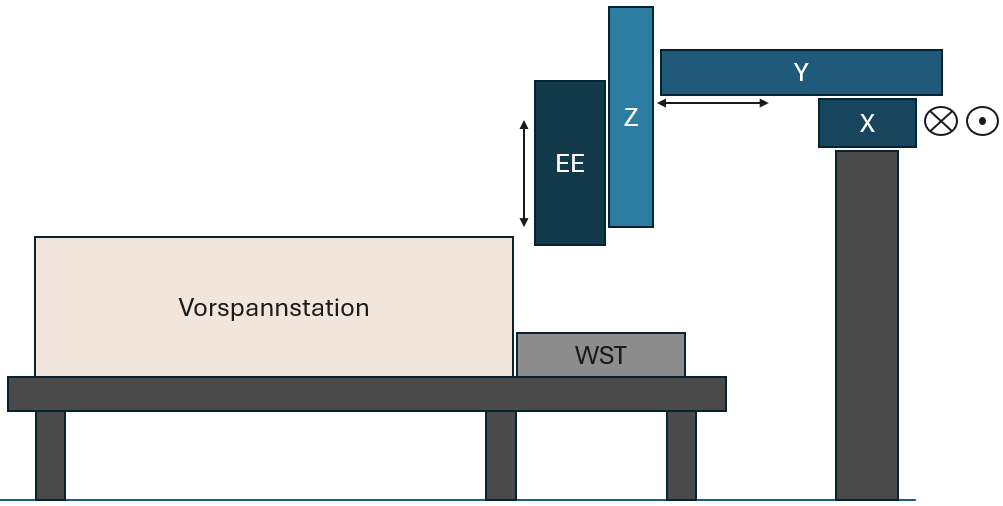
\includegraphics[width=0.8\linewidth]{Bilder/04_Konzeptentwicklung/Konzept_A.png}
    \caption{Zeichnung der Konzept A}
    \label{fig:concept_a}
\end{figure}

\textbf{Besonderheiten:}
\begin{itemize}
    \item Kartesische XYZ-Kinematik mit feststehender Vorspannstation
    \item Zugriff des Endeffektors von oben bzw. seitlich
    \item Klare Trennung zwischen Struktur, Kinematik und Prozessmodul
    \item Modularer Aufbau mit eindeutig definierten Achsen
\end{itemize}

\textbf{Vorteile:}
\begin{itemize}
    \item Hohe Positioniergenauigkeit durch einfache kartesische Bewegungen
    \item Gute Reproduzierbarkeit der Vorspann- und Schraubprozesse
    \item Hoher Automatisierungsgrad möglich
    \item Einfache Integration von Sensorik und Werkzeugen
    \item Hohe Wartungs- und Diagnosefreundlichkeit durch modularen Aufbau mit klar abgegrenzten, funktionsspezifischen Baugruppen
\end{itemize}

\textbf{Nachteile:}
\begin{itemize}
    \item Relativ hoher Platzbedarf, insbesondere in Z-Richtung
    \item Höherer konstruktiver Aufwand für ausreichende Steifigkeit
\end{itemize}

\paragraph{Konzeptvariante B:}
Konzeptvariante B stellt einen Kompromiss zwischen einem erhöhten Automatisierungsgrad und einer noch beherrschbaren Systemkomplexität dar.

Für diese Variante ist der Einsatz der P-50-Montageanlage der SmarAct Automation vorgesehen. Diese Anlage bietet einen hohen Integrationsgrad sowie einen hochpräzisen Gantry-Linearantrieb.\cite{SmarActAutomation_P50} Die Werkstückaufnahme erfolgt weiterhin manuell, während die Sicherung des Werkstücks über eine vakuumbasierte Aufnahme realisiert wird. Das Vorspannsystem basiert auch hier auf dem bereits bestehenden mechanischen System.

Die Erfassung der Schlittenposition erfolgt kamerabasiert, wodurch eine flexible und berührungslose Positionsbestimmung ermöglicht wird. Die Bewegung des Schraubwerkzeugs wird über ein Gantry-System umgesetzt. Das Einpressen der Einklappfedern erfolgt mittels einer ventilgesteuerten Presse. Der Schraubprozess wird mit einem drehmomentgeregelten MITO-Schrauber realisiert. Für Schiebebewegungen kommt ein Stift mit Gummiabdeckung zum Einsatz.

Als Endeffektor wird eine Mehrfach-Endeffektorlösung verwendet. Die Positionsüberwachung erfolgt über Encoder. Die Steuerung basiert auf einem IPC-basierten System. Die Station ist rollbar ausgeführt und verfügt über eine intelligente Abschaltung zur Reduzierung des Energieverbrauchs in Stillstandszeiten.

Im Vergleich zu Konzept A ist der technische Funktionsumfang deutlich erweitert. Gleichzeitig ist der Einsatz der P-50-Anlage mit einem erheblichen Investitionsaufwand verbunden, was diese Variante insbesondere aus wirtschaftlicher Sicht kritisch macht.

\begin{figure}[htbp]
    \centering
    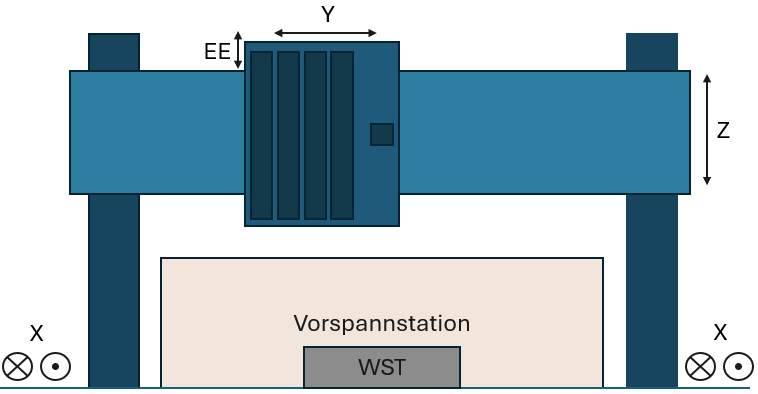
\includegraphics[width=0.8\linewidth]{Bilder/04_Konzeptentwicklung/Konzept_B.png}
    \caption{Zeichnung der Konzept B}
    \label{fig:concept_b}
\end{figure}

\textbf{Besonderheiten:}
\begin{itemize}
    \item Brückenförmiger Aufbau mit verfahrbarem Querträger
    \item Vorspannstation vollständig frei und stationär
    \item Kartesische Kinematik mit großem nutzbaren Arbeitsraum
    \item Zugriff von oben auf den Prozess
    \item Einsatz einer bestehenden Automationsplattform (P-50 aus SmarAct Automation) vorgesehen
\end{itemize}

\textbf{Vorteile:}
\begin{itemize}
    \item Deutlich reduzierter Konstruktions- und Entwicklungsaufwand durch die Nutzung einer vorhandenen Automationsanlage
    \item Hohe Integrationssicherheit durch erprobte Hardware und bestehende Schnittstellen
    \item Gute Eignung für teil- oder vollautomatisierte Prozesse
\end{itemize}

\textbf{Nachteile:}
\begin{itemize}
    \item Hoher Platzbedarf in der Fläche
    \item Sehr hohe Investitionskosten durch die Verwendung der SmarAct Automation P-50
    \item Wirtschaftlich nur bedingt sinnvoll für kleine Stückzahlen
    \item Geringere Freiheitsgrade bei der mechanischen Anpassung im Vergleich zu einer Eigenkonstruktion
\end{itemize}

\paragraph{Konzeptvariante C:}
Konzeptvariante C verfolgt einen deutlich stärkeren automatisierten und modularen Ansatz. Ziel ist eine hohe Flexibilität und Zukunftssicherheit, auch bei erhöhtem technischem und organisatorischem Aufwand.

Die Werkstückaufnahme erfolgt manuell, und die Sicherung erfolgt über eine mechanische Spannvorrichtung. Die Baugrößenumschaltung wird automatisch durch das Einlesen eines Data-Matrix-Codes realisiert. Für die Vorspannung wird weiterhin das bestehende mechanische Vorspannsystem verwendet.

Die Schlittenposition wird mittels eines Laser-Triangulationssensors erfasst. Die Bewegung des Schraubwerkzeugs erfolgt über ein Pick-and-Place-System. Das Einpressen der Einklappfedern wird durch eine servogetriebene Mini-Presse umgesetzt. Der Schraubprozess erfolgt auch hier mit einem drehmomentgeregelten MITO-Schrauber. Für Schiebebewegungen wird ein aufsteckbares Gummipad an der Presse eingesetzt.

Als Endeffektor kommt ein einfacher Greifer zum Einsatz. Die Positionsüberwachung erfolgt über Encoder. Die Steuerung basiert auf einem Industrie-Robotercontroller. Die Station ist modular zerlegbar ausgeführt und verfügt über eine intelligente Abschaltung zur Verbesserung der Energieeffizienz.

\begin{figure}[htbp]
    \centering
    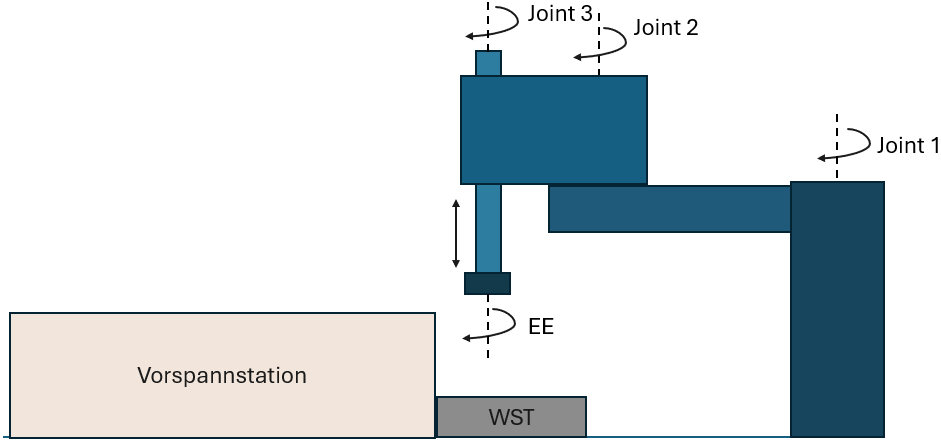
\includegraphics[width=0.8\linewidth]{Bilder/04_Konzeptentwicklung/Konzept_C.png}
    \caption{Zeichnung der Konzept C}
    \label{fig:concept_c}
\end{figure}

\textbf{Besonderheiten:}
\begin{itemize}
    \item Einsatz eines SCARA- bzw. SCARA-artigen Roboters als zentrale Kinematik
    \item Der Endeffektor greift einzelne Werkzeuge
    \item Die Bearbeitung erfolgt durch das jeweils aufgenommene Modul; danach wird es wieder zurückgelegt
    \item Der Roboter übernimmt damit sowohl die Handhabung (Greifen/Positionieren) als auch die Prozessausführung (Schrauben, Einpressen, Verschieben)
    \item Prozessmodule sind als wechselbare Einheiten ausgeführt (modulares Werkzeugkonzept)
\end{itemize}

\textbf{Vorteile:}
\begin{itemize}
    \item Hohe Flexibilität: unterschiedliche Prozessschritte können über verschiedene Module abgedeckt werden
    \item Geringer Bauraumbedarf im Vergleich zu Portal/Gantry, da keine große Brückenstruktur nötig ist
    \item Modular erweiterbar: neue Prozessmodule können ergänzt werden, ohne die gesamte Mechanik zu ändern
    \item Gute Eignung für Variantenfähigkeit (SLC / SLC-W) durch wechselbare Werkzeuge
\end{itemize}

\textbf{Nachteile:}
\begin{itemize}
    \item Höherer Steuerungs- und Integrationsaufwand
    \item Reproduzierbarkeit kritisch, weil Werkzeugaufnahme und Rückgabe Toleranzen einbringen
    \item Genauigkeit/Stabilität unter Prozesskräften kann schlechter sein als bei kartesischen Achsen
    \item Zusätzliche Risiken durch Kollisionen und komplexere Sicherheitsbetrachtungen
\end{itemize}

\subsection{Konzeptbewertung}
\subsubsection{Bewertungskriterien}
\label{sec:Bewertungskriterien}
Zur vergleichenden Bewertung der entwickelten Konzeptvarianten wurden geeignete Bewertungskriterien festgelegt, die sowohl technische als auch wirtschaftliche und organisatorische Aspekte des Systems abdecken. Ziel ist es, eine nachvollziehbare und möglichst objektive Entscheidungsgrundlage für die Auswahl eines Vorzugskonzepts zu schaffen.\cite{MKon_VL, ZangemeisterNutzwertanalyse}

Die Gewichtung der Bewertungskriterien erfolgte mithilfe eines Paarvergleichs. Dabei wurden die einzelnen Kriterien jeweils paarweise gegenübergestellt und hinsichtlich ihrer relativen Bedeutung für die Zielsetzung des Systems bewertet. Dieses Vorgehen ermöglicht es, subjektive Einzelmeinungen zu reduzieren und die Wichtigkeit der Kriterien systematisch und transparent abzuleiten.\cite{MKon_VL, ZangemeisterNutzwertanalyse}

Für den Paarvergleich wurde ein dreistufiges Bewertungsschema verwendet. Ein Wert von 2 bedeutet, dass ein Kriterium gegenüber dem Vergleichskriterium deutlich wichtiger ist. Ein Wert von 1 kennzeichnet eine gleichwertige Bedeutung beider Kriterien. Ein Wert von 0 wird vergeben, wenn das betrachtete Kriterium weniger wichtig ist als das gegenübergestellte.

Als Bewertungskriterien wurden folgende Aspekte definiert: Funktionalität, Robustheit, Montierbarkeit, Präzision, Kosten, Automatisierungsgrad, Effizienz und Zeit sowie Ästhetik. Diese Kriterien spiegeln die wesentlichen Anforderungen an die Montagestation wider und berücksichtigen sowohl den technischen Nutzen als auch praktische Gesichtspunkte der Umsetzung.

Aus der Summierung der Bewertungen ergibt sich für jedes Kriterium eine Zeilensumme, aus der anschließend die prozentuale Gewichtung berechnet wurde. Die prozentualen Anteile geben die relative Bedeutung der einzelnen Kriterien innerhalb der Nutzwertanalyse wieder. Zusätzlich wurde auf Basis dieser Gewichtung eine Rangfolge der Kriterien erstellt.

Die Ergebnisse des Paarvergleichs zeigen, dass insbesondere die Kriterien Funktionalität und Präzision eine hohe Bedeutung für die Bewertung der Konzepte besitzen. Ebenfalls relevant sind der Automatisierungsgrad sowie Aspekte der Effizienz und Prozesszeit. Kriterien wie Montierbarkeit, Kosten und Ästhetik wurden zwar berücksichtigt, weisen jedoch im Vergleich eine geringere Gewichtung auf.

Die so ermittelten Gewichtungsfaktoren bilden die Grundlage für die nachfolgende Nutzwertanalyse und fließen direkt in die Bewertung der einzelnen Konzeptvarianten ein.

{
\begin{table}[H]
\centering
\small
\setlength{\tabcolsep}{4pt}
\renewcommand{\arraystretch}{1.2}

\begin{tabular}{|l|c|c|c|c|c|c|c|c|c|c|c|}
\hline
 & \rotatebox{90}{Funktionalität} & \rotatebox{90}{Robustheit} & \rotatebox{90}{Montierbarkeit} &
 \rotatebox{90}{Präzision} & \rotatebox{90}{Kosten} & \rotatebox{90}{Automatisierungsgrad} &
 \rotatebox{90}{Effizienz und Zeit} & \rotatebox{90}{Ästhetik} &
 \rotatebox{90}{Zeilensumme} & \rotatebox{90}{\%} & \rotatebox{90}{Rang} \\
\hline
Funktionalität        & \textbf{X} & 2 & 2 & 1 & 2 & 2 & 2 & 2 & 13 & 23,21 & 1 \\
\hline
Robustheit            & 0 & \textbf{X} & 2 & 0 & 2 & 0 & 1 & 2 & 7  & 12,50 & 4 \\
\hline
Montierbarkeit        & 0 & 0 & \textbf{X} & 0 & 2 & 0 & 0 & 1 & 3  & 5,36  & 6 \\
\hline
Präzision             & 1 & 2 & 2 & \textbf{X} & 2 & 1 & 2 & 1 & 11 & 19,64 & 2 \\
\hline
Kosten                & 0 & 0 & 0 & 0 & \textbf{X} & 1 & 1 & 2 & 4  & 7,14  & 5 \\
\hline
Automatisierungsgrad  & 0 & 2 & 2 & 1 & 1 & \textbf{X} & 1 & 2 & 9  & 16,07 & 3 \\
\hline
Effizienz und Zeit    & 0 & 1 & 2 & 0 & 1 & 1 & \textbf{X} & 2 & 7  & 12,50 & 4 \\
\hline
Ästhetik              & 0 & 0 & 1 & 1 & 0 & 0 & 0 & \textbf{X} & 2  & 3,57  & 7 \\
\hline
\textbf{SUMME} & \textbf{X} & \textbf{X} & \textbf{X} & \textbf{X} & \textbf{X} & \textbf{X} & \textbf{X} & \textbf{X} & \textbf{56} & \textbf{100,00} & X \\
\hline
\end{tabular}

\caption{Paarvergleich zur Gewichtung der Bewertungskriterien für die Nutzwertanalyse}
\label{tab:bewertungskriterien_paarvergleich}
\end{table}
}

\subsubsection{Durchführung der Nutzwertanalyse}
Zur vergleichenden Bewertung der entwickelten Konzeptvarianten wurde eine Nutzwertanalyse durchgeführt. Grundlage hierfür bilden die in Abschnitt~\ref{sec:Bewertungskriterien} definierten und gewichteten Bewertungskriterien. Ziel der Nutzwertanalyse ist es, die unterschiedlichen Konzepte anhand einheitlicher Maßstäbe quantitativ miteinander zu vergleichen und so eine fundierte Entscheidungsbasis für die Auswahl eines Vorzugskonzepts zu schaffen.

Jede Konzeptvariante wurde für jedes Bewertungskriterium mit einer Punktzahl auf einer Skala von 1 bis 5 bewertet. Dabei steht der Wert 1 für eine sehr geringe Erfüllung des jeweiligen Kriteriums, während der Wert 5 eine sehr gute Erfüllung beschreibt. Die Bewertung erfolgte auf Basis der zuvor beschriebenen konzeptionellen Ausprägungen der Varianten sowie unter Berücksichtigung der technischen Machbarkeit, Systemkomplexität und des zu erwartenden Aufwands.

Zur Berechnung des Nutzwerts wurde die jeweilige Bewertung mit dem Gewichtungsfaktor des entsprechenden Kriteriums multipliziert. Auf diese Weise ergibt sich für jedes Kriterium ein gewichteter Teilwert. Die Summe aller gewichteten Teilwerte bildet den Gesamtnutzwert der jeweiligen Konzeptvariante.

Durch dieses Vorgehen wird sichergestellt, dass Kriterien von hoher Bedeutung, wie Funktionalität oder Präzision, stärker in das Gesamtergebnis einfließen als weniger gewichtete Kriterien. Gleichzeitig erlaubt die Nutzwertanalyse einen transparenten Vergleich der Konzepte, da sowohl Einzelbewertungen als auch deren Gewichtung nachvollziehbar dargestellt sind.

Die Ergebnisse der Nutzwertanalyse sind in Tabelle~\ref{tab:nutzwertanalyse} zusammengefasst.

{
\begin{table}[H]
\centering
\small
\setlength{\tabcolsep}{4pt}
\renewcommand{\arraystretch}{1.2}

\begin{tabular}{|l|c|c|c|c|c|c|c|}
\hline
\multirow{2}{*}{\textbf{Kriterium}} &
\multirow{2}{*}{\textbf{Faktor (\%)}} &
\multicolumn{2}{c|}{\textbf{Konzept 1}} &
\multicolumn{2}{c|}{\textbf{Konzept 2}} &
\multicolumn{2}{c|}{\textbf{Konzept 3}} \\
\cline{3-8}
 &  & \textbf{Bew.} & \textbf{Wert} & \textbf{Bew.} & \textbf{Wert} & \textbf{Bew.} & \textbf{Wert} \\
\hline
Funktionalität       & 23,21 & 5 & 116,07 & 5 & 116,07 & 4 & 92,86 \\
\hline
Robustheit           & 12,50 & 5 & 62,50  & 5 & 62,50  & 4 & 50,00 \\
\hline
Montierbarkeit       & 5,36  & 5 & 26,79  & 4 & 21,43  & 5 & 26,79 \\
\hline
Präzision            & 19,64 & 4 & 78,57  & 5 & 98,21  & 2 & 39,29 \\
\hline
Kosten               & 7,14  & 5 & 35,71  & 1 & 7,14   & 3 & 21,43 \\
\hline
Automatisierungsgrad & 16,07 & 3 & 48,21  & 3 & 48,21  & 3 & 48,21 \\
\hline
Effizienz und Zeit   & 12,50 & 5 & 62,50  & 4 & 50,00  & 1 & 12,50 \\
\hline
Ästhetik             & 3,57  & 3 & 10,71  & 4 & 14,29  & 3 & 10,71 \\
\hline
\textbf{SUMME} & \textbf{100,00} &  & \textbf{441,07} &  & \textbf{417,86} &  & \textbf{301,79} \\
\hline
\end{tabular}

\caption{Nutzwertanalyse der Konzeptvarianten}
\label{tab:nutzwertanalyse}
\end{table}
}

\subsubsection{Auswahl des Vorzugskonzepts}
Auf der Grundlage der durchgeführten Nutzwertanalyse lassen sich die Konzeptvarianten eindeutig miteinander vergleichen.

Das hohe Ergebnis von Konzept A ist insbesondere auf die sehr guten Bewertungen in den hoch gewichteten Kriterien Funktionalität, Präzision sowie Effizienz und Zeit zurückzuführen. Zudem weist diese Variante eine gute Kostenbewertung auf, was sich positiv auf den Gesamtnutzwert auswirkt. Insgesamt zeigt sich ein ausgewogenes Verhältnis zwischen technischer Leistungsfähigkeit und Systemaufwand.

Konzept B erzielt gute Ergebnisse in den Bereichen Präzision und Funktionalität, weist jedoch deutliche Nachteile bei den Kosten auf. Der hohe Investitionsaufwand, insbesondere durch den Einsatz einer hochintegrierten industriellen Montageanlage, wirkt sich trotz technischer Vorteile negativ auf das Gesamtergebnis aus.

Konzept C erreicht ebenfalls hohe Bewertungen in einzelnen technischen Kriterien, insbesondere in der Präzision. Allerdings führen der erhöhte Automatisierungs- und Integrationsaufwand sowie geringere Bewertungen in den Bereichen Effizienz und Kosten zu einem vergleichsweise niedrigen Gesamtnutzwert.

Aufgrund des höchsten Gesamtnutzwerts und des ausgewogenen Verhältnisses zwischen Nutzen, Aufwand und Umsetzbarkeit wird Konzept A als Vorzugskonzept ausgewählt und im weiteren Verlauf der Arbeit detailliert ausgearbeitet.